%% copy made Jan 3, 2022
%\setcounter{chapter}{4}        
\chapter{Stereo}

Figure~\ref{fig:lunarRocks}~(a) shows a stereo pair image of lunar rocks, photographed by Neil Armstrong during the first manned mission to the Moon \cite{apolloStereo}.  The displacement of the camera views creates a sense of depth when the left and right images are displayed separately to our left and right eyes.  This sense of depth can also be observed by toggling between the two overlaid images in the
%% https://groups.csail.mit.edu/vision/cvbook/videos/A11wigglestereo6712.gif
\href{https://groups.csail.mit.edu/vision/cvbook/videos/A11wigglestereo6712.gif}{"wiggleview" gif}, (b).  In this chapter, we study how to compute depth from a pair of spatially offset camera images, such as those of Fig.~\ref{fig:lunarRocks}.

\begin{figure}
\centerline{
\sublabelnp{(a) stereo pair}{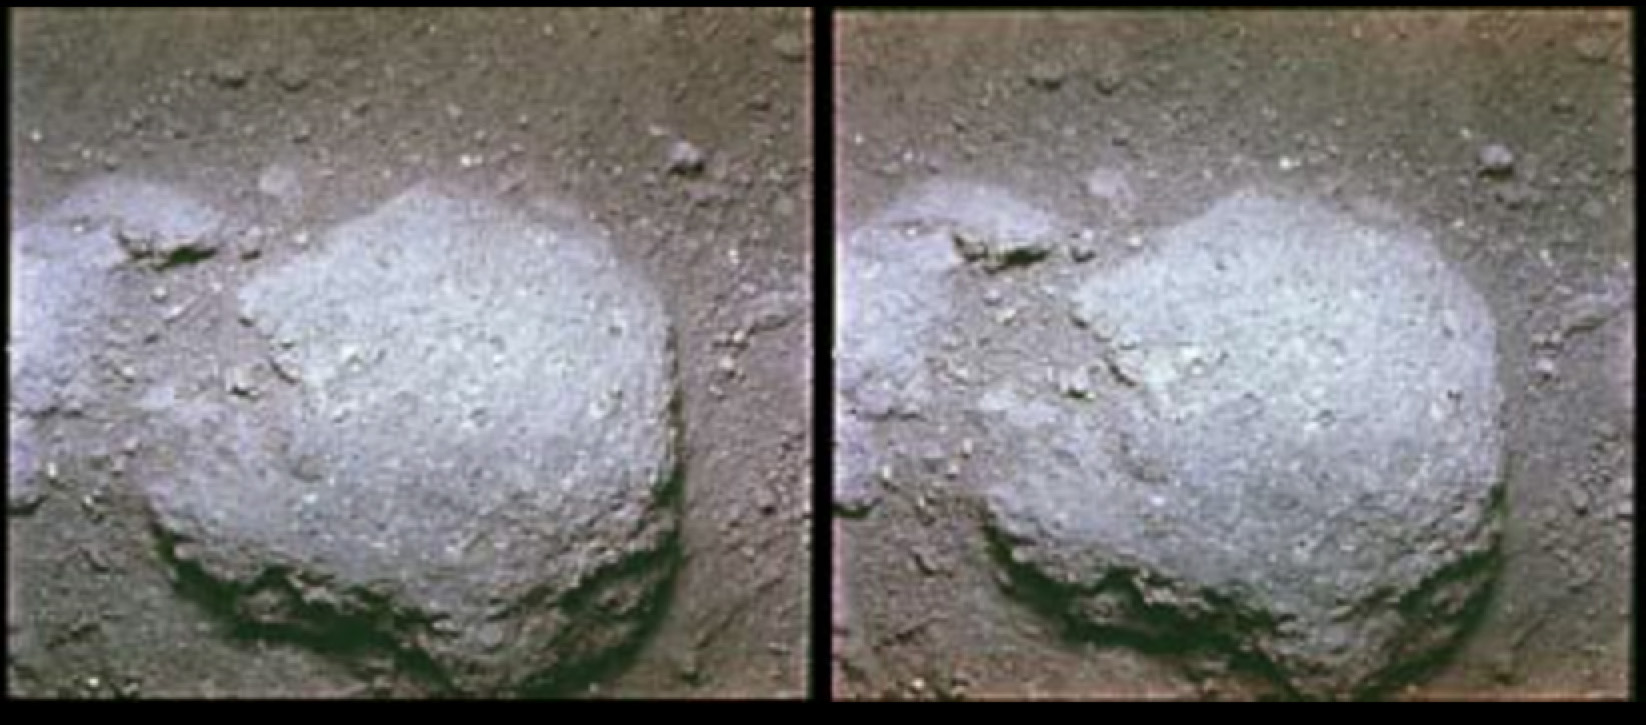
\includegraphics[width=0.6\linewidth]{figures/stereo/stereoLunarRocks.jpg}}
\sublabelnp{(b) 
\href{https://groups.csail.mit.edu/vision/cvbook/videos/A11wigglestereo6712.gif}{Wiggleview gif animation}
}{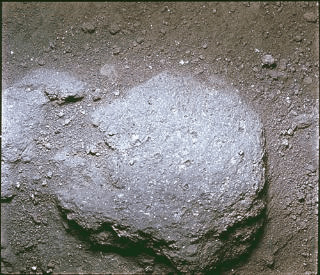
\includegraphics[width=0.3\linewidth]{figures/stereo/wiggle.jpg}}
}
\caption{(a) Stereo images of lunar rocks taken during Apollo 11 mission, from \cite{nasaApollo11}.  (b) Wiggleview of this stereo pair \href{https://groups.csail.mit.edu/vision/cvbook/videos/A11wigglestereo6712.gif}{(click for animation)}.}
\label{fig:lunarRocks}
\end{figure}


\section{Stereo triangulation}


\begin{figure}
\centerline{
\sublabel{a}{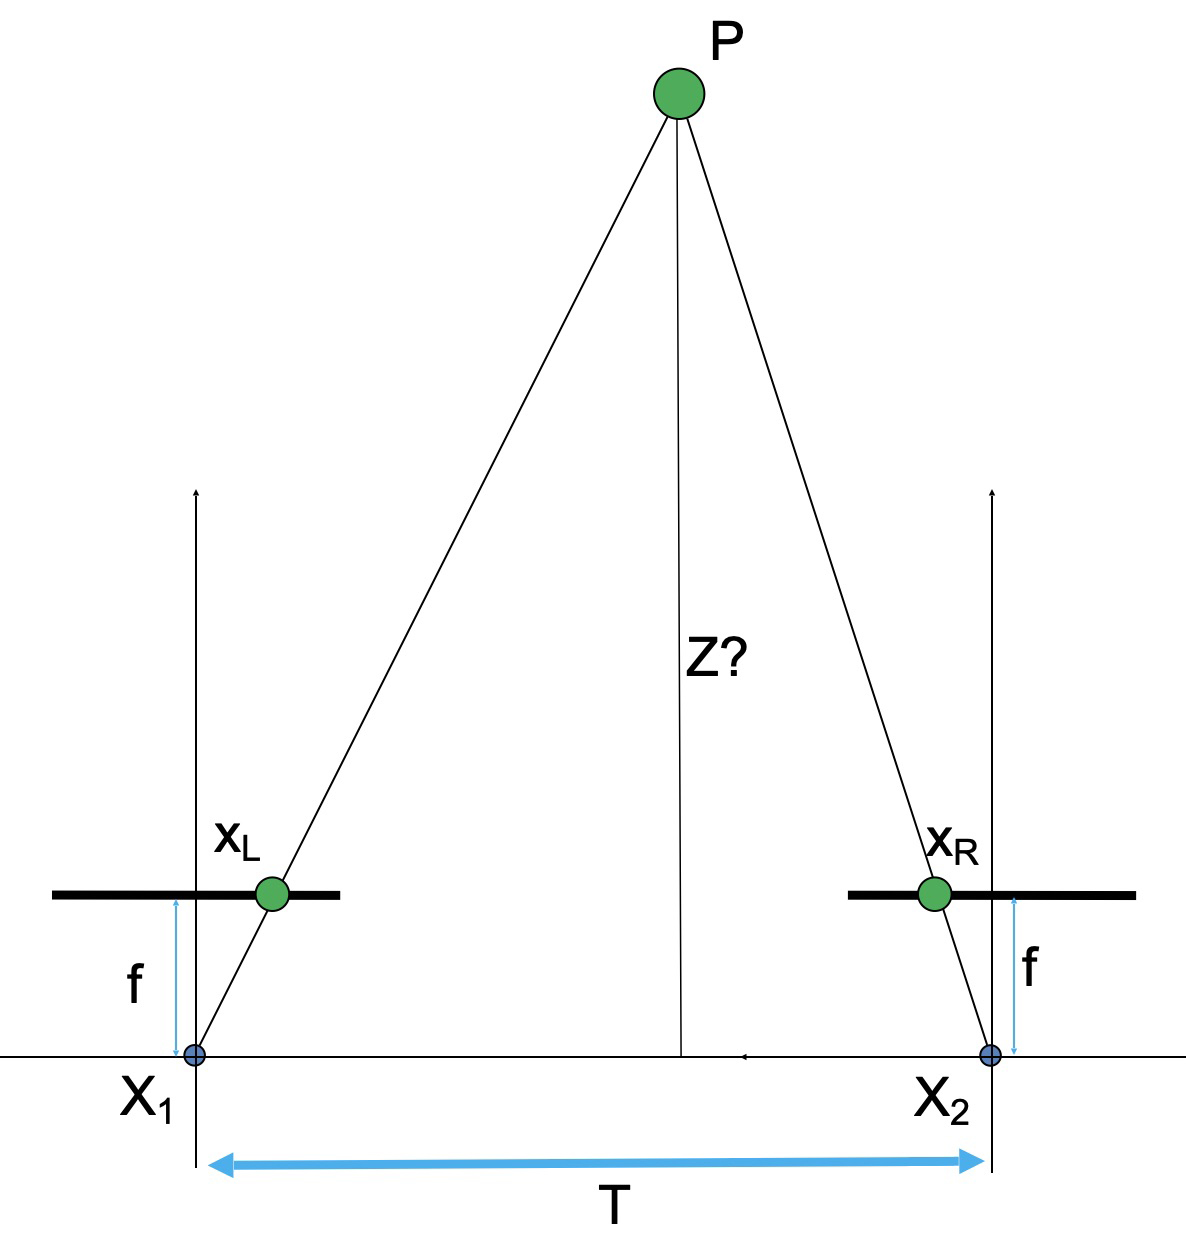
\includegraphics[width=0.4\linewidth]{figures/stereo/stereo.jpg}}}
\centerline{
\sublabel{b}{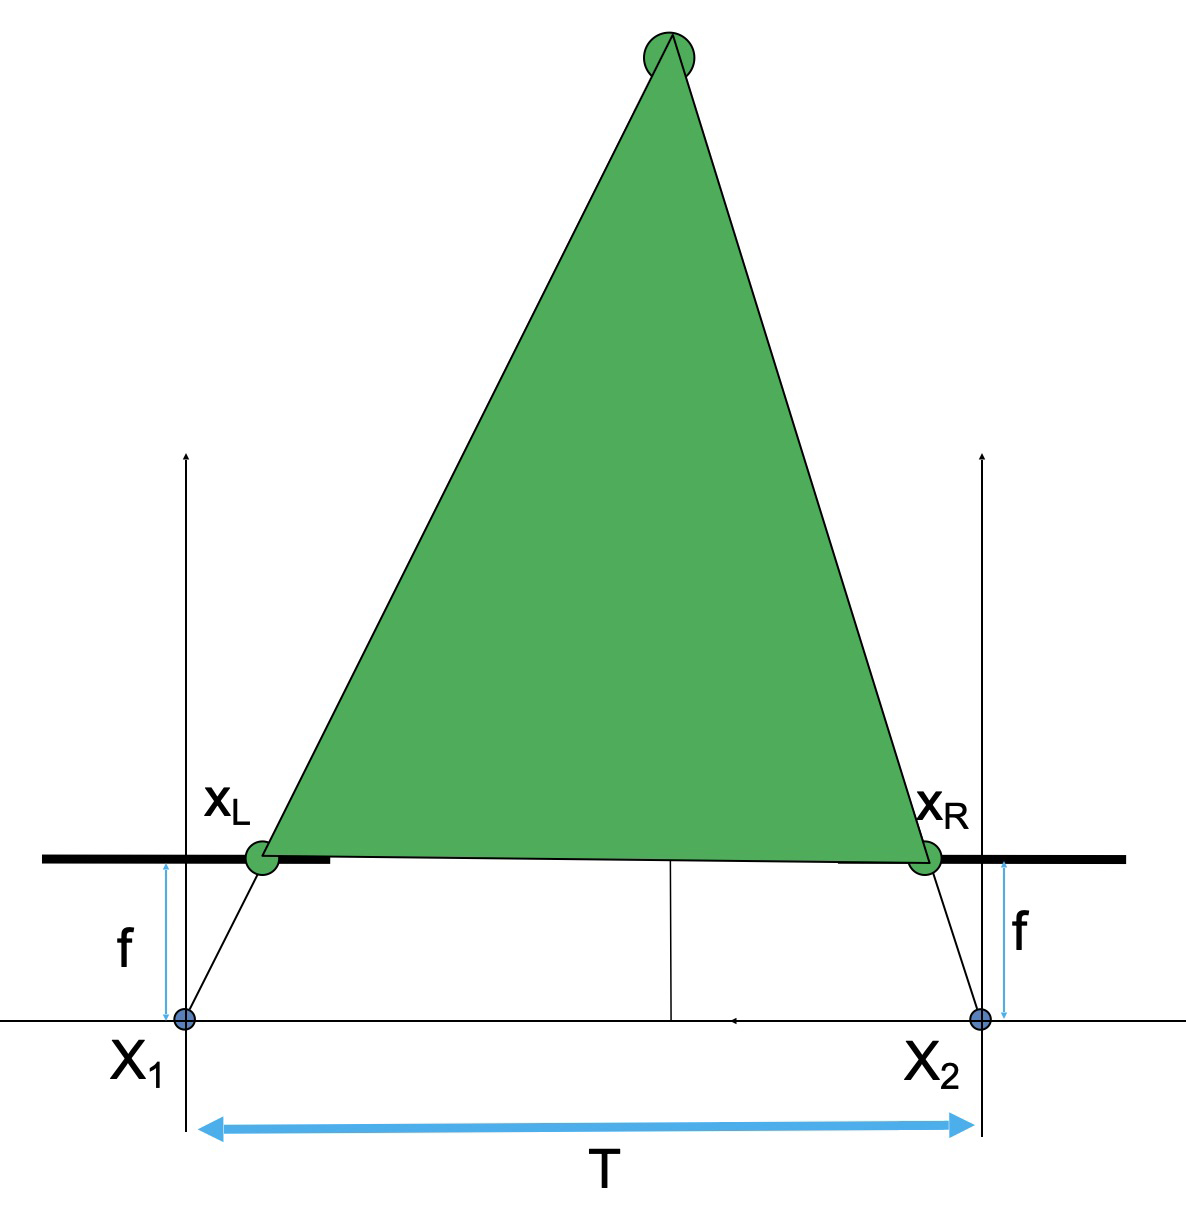
\includegraphics[width=0.4\linewidth]{figures/stereo/stereoGreen.jpg}}
\sublabel{c}{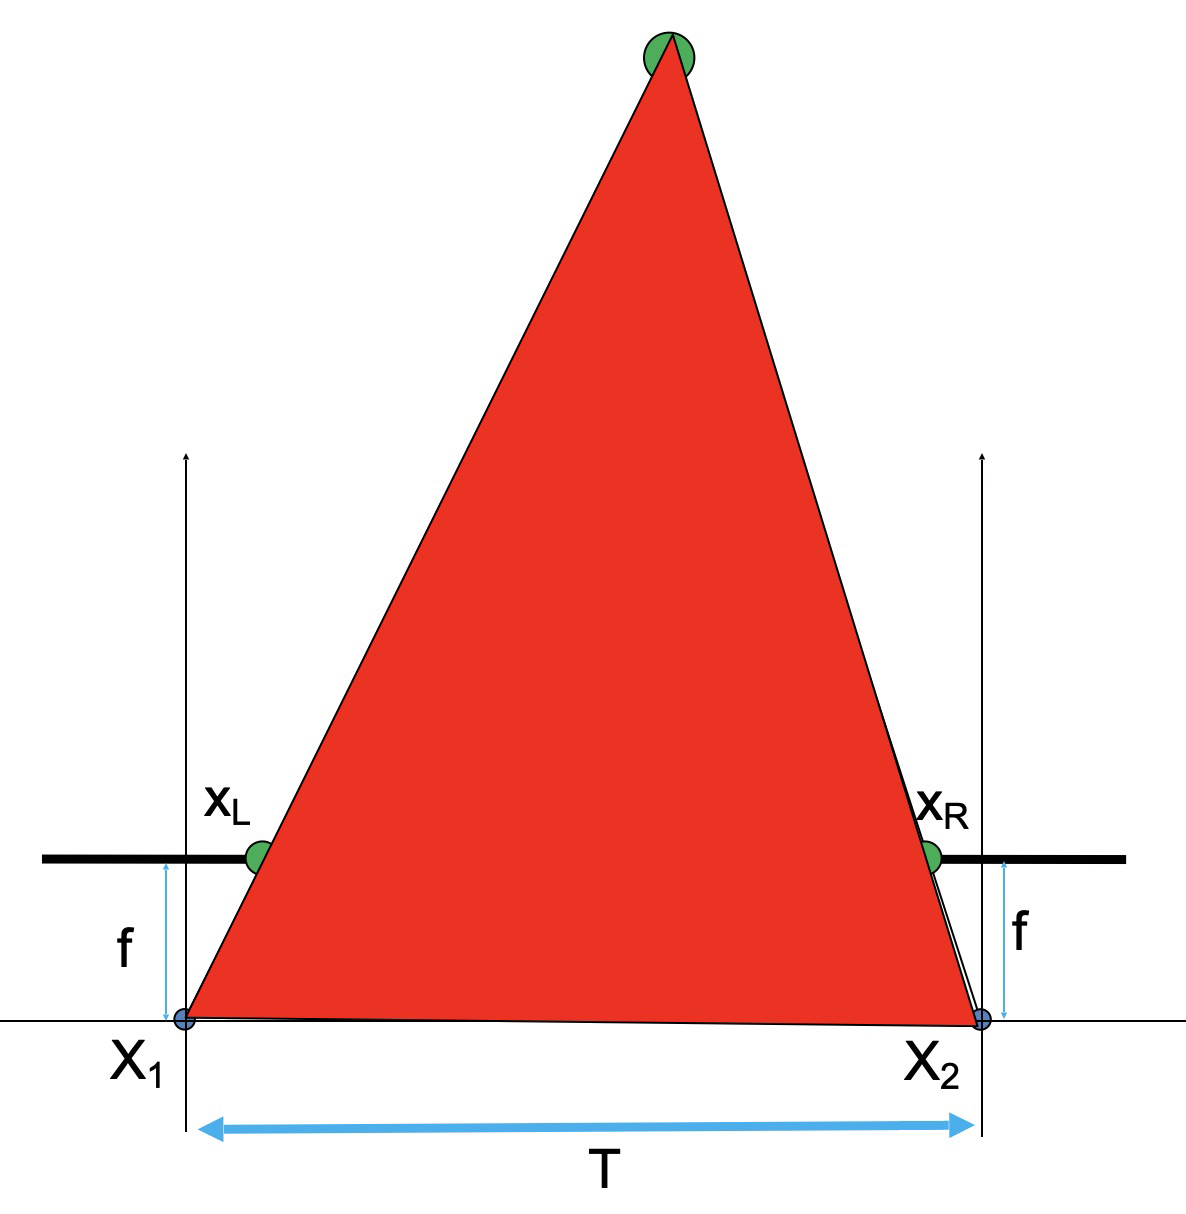
\includegraphics[width=0.4\linewidth]{figures/stereo/stereoRed.jpg}}
}
\caption{Depth triangulation from stereo. (a) Two cameras, of identical focal length, f, and separated by an offset, T, image the point P onto $X_1$ and $X_2$ at camera.  The similarity of the two triangles in (b) and (c) leads to Eq.~(\ref{eq:depthFromDisparity}) for the depth, Z, of the point P.}
\label{fig:stereo}
\end{figure}

The task of stereo is to triangulate the depth of points in the world by comparing the images from two spatially offset cameras.  (If more than two cameras are used, the task is referred to as multi-view stereo).  To derive stereo algorithms, we need to describe how the spatial positions of points in image relate to their corresponding positions in the 3d world. 
The algorithms to compute depth from two stereo cameras are  simplified if we assume a special relationship between the two cameras:  first, that they are identical, and, further, are identically oriented in space, differing only by a horizontal translation between the two cameras, ie, a translation parallel to the rows each image.  Later in this chapter, we will allow a more general relationship between the cameras by developing a stereo pre-processing step called {\bf rectification}.  Rectification warps one image of the stereo pair to synthesize the image that would have been recorded had the two cameras had the special relationship described above.


The simplified geometry shown in Fig.~\ref{fig:stereo} reveals the essence of depth estimation using a stereo pair of cameras.  The two cameras are centered  at horizontal positions $X_1$ and $X_2$, respectively, and are identical and are oriented with their optical axes parallel with each other.   (To distinguish 2d image coordinates from 3d world coordinates, for this chapter, we will denote 2-d image coordinates by lower-case letters, and 3-d world coordinates by upper-case letters.) The green circle at point P, for which we want to estimate the depth, Z, appears in the left camera at position $X_L$ and in the right camera at position $X_R$.  

A simple way to triangulate the depth, Z, of a point visible in both images is through similar triangles.  The two triangles shown in  Fig.~\ref{fig:stereo}~(b) and (c) are similar, and so the ratios of their height to base must be the same.  Thus we have:
\begin{equation}
    \frac{T+X_R-X_L}{Z-f} = \frac{T}{Z}
\end{equation}
Solving for Z gives:
\begin{equation}
    Z = f \frac{T}{X_L-X_R}
    \label{eq:depthFromDisparity}
\end{equation}
The difference in horizontal position of the point in the left and right camera views, $X_L - X_R$, is called the {\bf disparity}, and is inversely proportional to the depth Z of the point P.

To find the depth of every point visible in both images of a stereo pair, we must localize corresponding points in each image, and compute the disparity between their positions in the left and right images. So the general tasks of stereo algorithm are

\begin{enumerate}
    \item Image Rectification (we delay this to Sect.~\ref{sect:epipolar}).
    \item Finding image features throughout both images of the stereo pair.
    \item Match the features found in one image to the corresponding features in the other image in order to calculate the stereo disparity, and thus the depth, of each feature point.
    \item Invoke assumptions about shapes in the world to compute the depths at positions between feature point locations.
\end{enumerate}


To measure the disparity that tells us depth, we need to find matching points over the two images of the stereo pair.  First, let's examine the task visually.   Figure~\ref{fig:stereomatch} shows two images of an office, take approximately one meter apart.  The locations of several objects in the left image, (a), are shown in the right image, (b), revealing some of the disparities that we seek to measure automatically.  As the reader can appreciate by comparing the stereo images by eye, one must first localize a feature point in one image, exploiting edges or textures, and then find the corresponding point in the other image, based on the visual similarity of the local image region.


\section{Finding image features}
Good image features are positions in the image that area easy to localize.  The Harris corner \cite{Harris88} algorithm identifies image points that are easy to localize by evaluating the sum of squared intensity differences over an image patch caused by a small translation of the image. If the squared intensity changes quickly with patch translation, then the region contains a good image feature. 

Let the image be $x[n,m]$, and let the small translation be $\delta n$ in $n$ and $\delta m$ in $m$.  Then the squared intensity difference, $E(\delta n, \delta m)$ induced by that small translation, summed over a small patch, will be
\begin{equation}
    E(\delta n, \delta m) = \Sigma_{(n, m) \in P}
    (x[n,m] - x[n + \delta n, m + \delta m])^2
    \label{eq:harris}
\end{equation}

We expand $x[n + \delta n, m + \delta m]$ about $x[n, m]$ in a Taylor series:
\begin{equation}
    x[n + \delta n, m + \delta m] \approx
    x[n, m] + \frac{\partial x}{\partial n} \delta n
    + \frac{\partial x}{\partial m} \delta m
\end{equation}
Substituting the above into Eq.~\ref{eq;harris} and writing the result in matrix form yields
\begin{equation}
       E(\delta n, \delta m) \approx
       \left( \begin{array}{c c}
       \delta n & \delta m
       \end{array}
       \right)
       \mathbf{M} 
       \left( \begin{array}{c}
       \delta n \\
       \delta m
       \end{array}
       \right) 
\end{equation}
where
\begin{equation}
M = \Sigma_{(n, m) \in P}
\left( \begin{array}{c c}
(\frac{\partial x}{\partial n})^2 & 
\frac{\partial x}{\partial n} 
\frac{\partial x}{\partial m} \\
\frac{\partial x}{\partial n} 
\frac{\partial x}{\partial m} 
& (\frac{\partial x}{\partial m})^2
\end{array} \right)
\end{equation}

matching and filtering stages.
%% https://arxiv.org/pdf/2109.07547.pdf

As for other vision tasks, neural network approaches now dominate stereo methods.
In modern neural-network-based approaches, the features are found by ...  (look at jia's paper for survey of approaches).




Intuitively, we know what each feature "looks like" visually, and so we can match them from one image to the other. We seek an automatic method to match image features between the two images.

 Harris features, based on edge and corner detection, \cite{Harris88} have been widely used, but later supplanted by SIFT features \cite{Lowe04}, based on maxima over scale of Laplacian filter outputs.  Figure~\ref{fig:stereopoints}~(a) and (b) show the result of the Harris feature detector to the images of Fig.~\ref{fig:stereomatch}.


\begin{figure}
\centerline{
\sublabel{a}{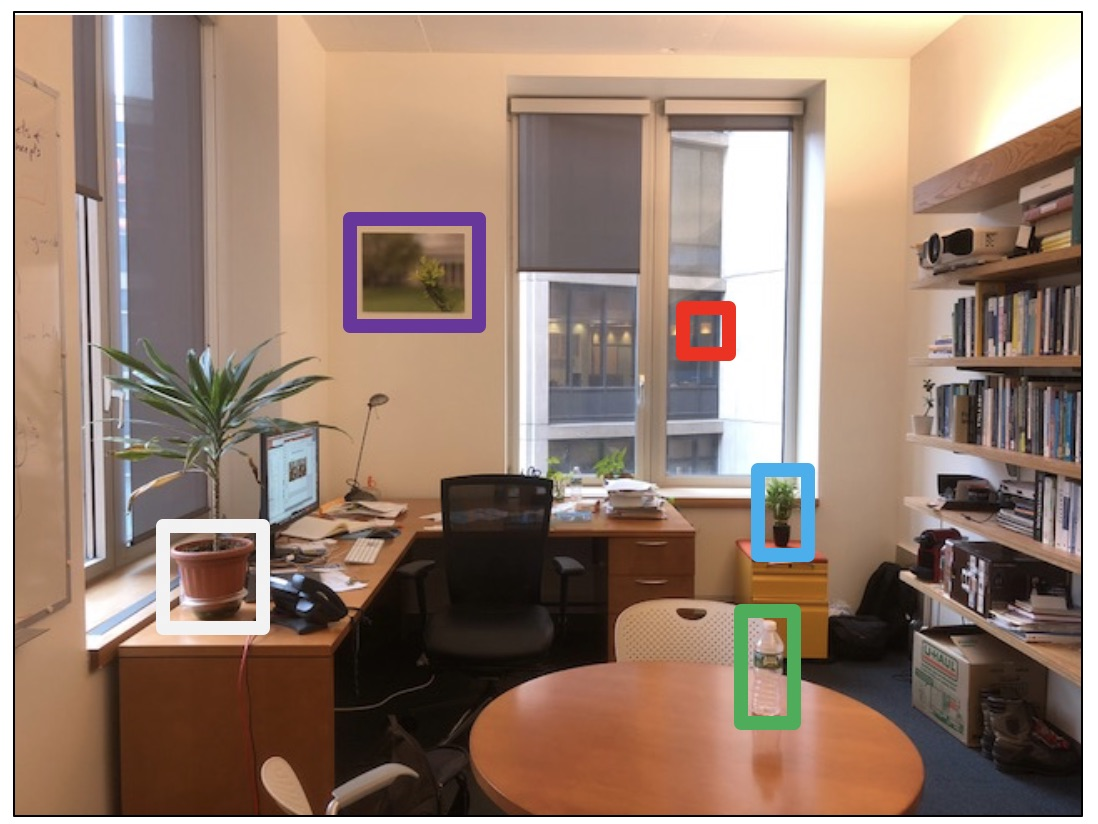
\includegraphics[width=0.4\linewidth]{figures/stereo/officeLeft.jpg}}
\sublabel{b}{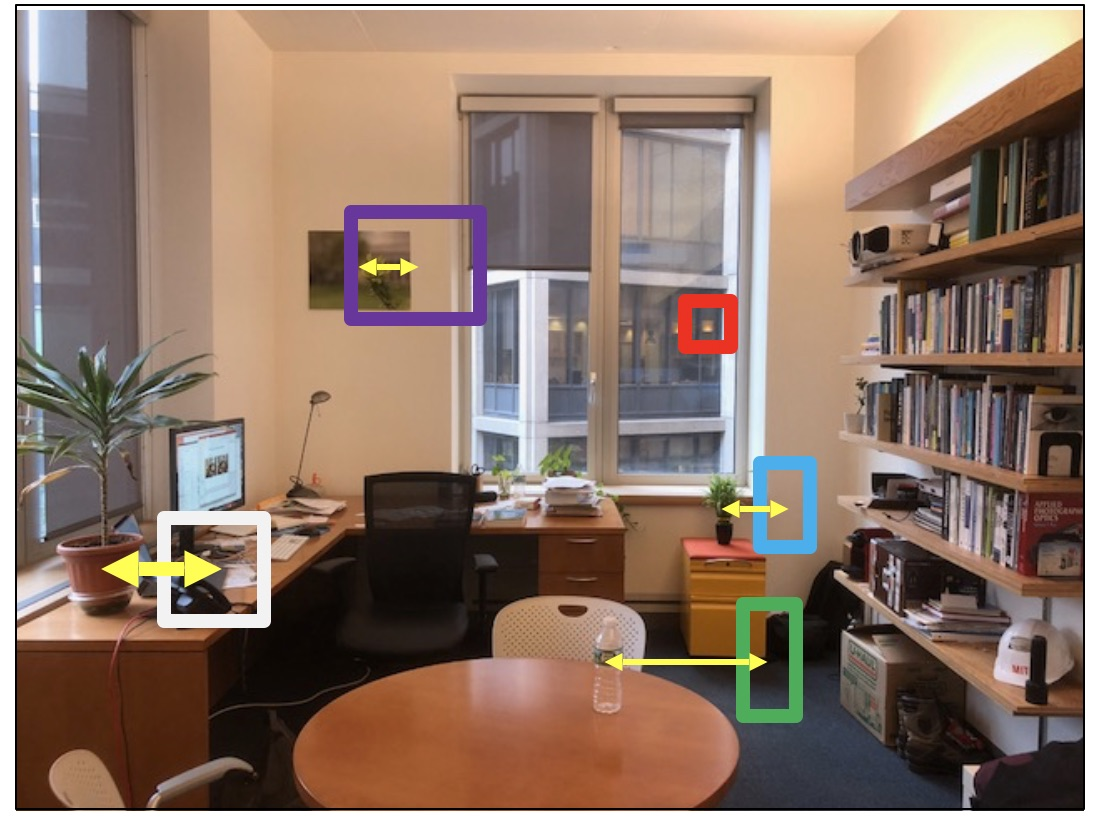
\includegraphics[width=0.4\linewidth]{figures/stereo/officeRight.jpg}}
}
\caption{Two cameras, displaced from each other laterally, photograph the same scene, resulting in images (a) and (b).  Colored rectangles show some identifiable features in image (s), and where those features appear in image (b).  Arrows show the corresponding displacement, which can reveal depth through Eq.~(\ref{eq:depthFromDisparity})}.
\label{fig:stereomatch}
\end{figure}

\begin{figure}
\centerline{
\sublabel{a}{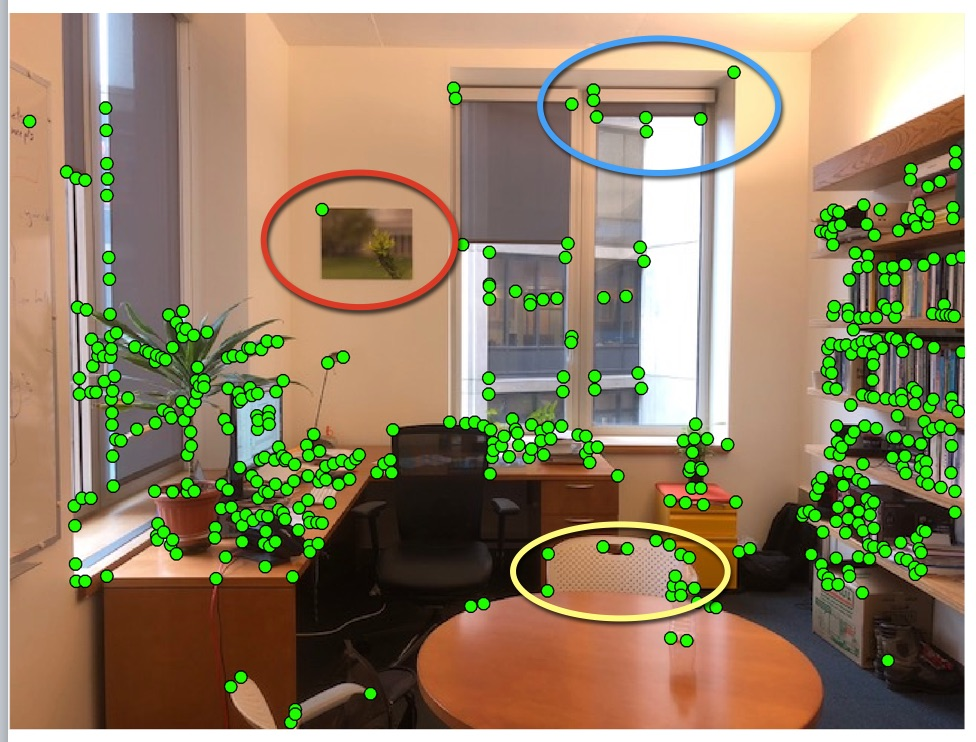
\includegraphics[width=0.4\linewidth]{figures/stereo/pointsLeft.jpg}}
\sublabel{b}{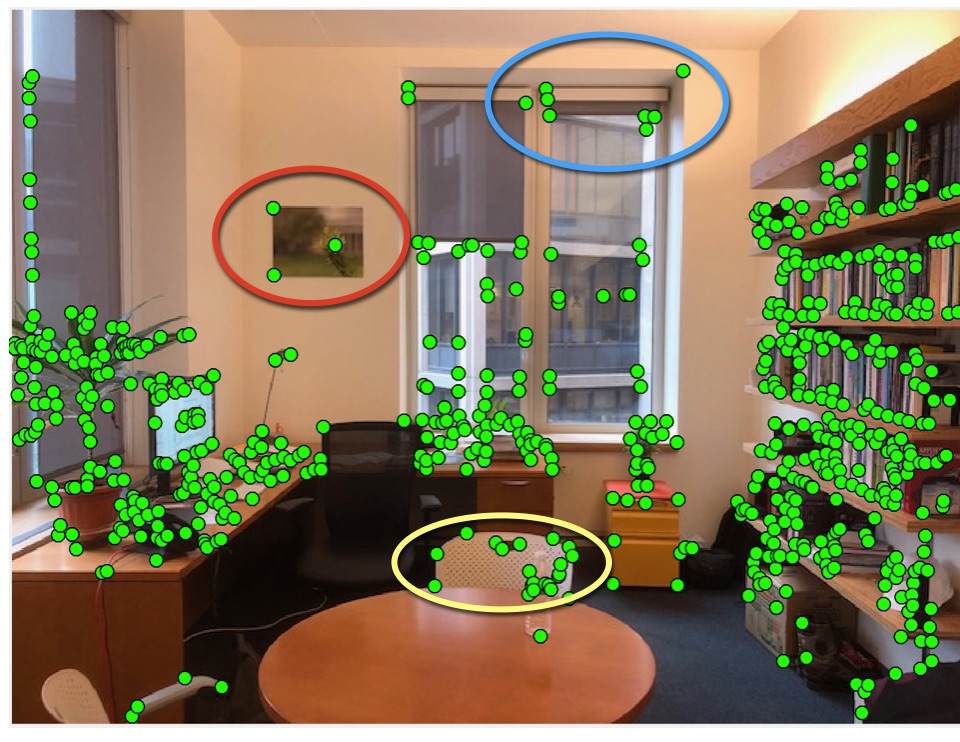
\includegraphics[width=0.4\linewidth]{figures/stereo/pointsRight.jpg}}
\sublabel{c}{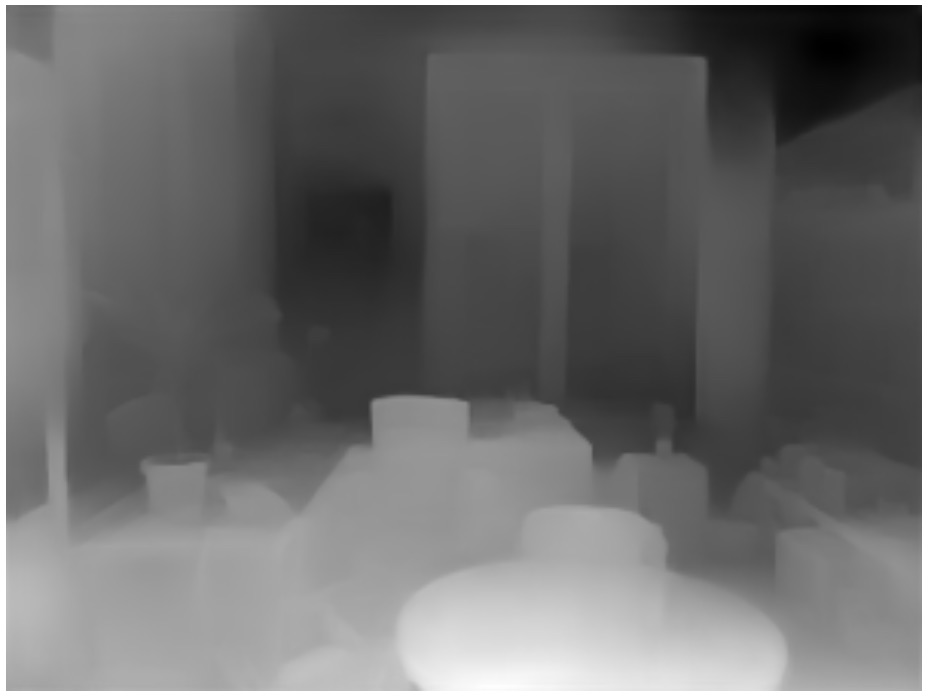
\includegraphics[width=0.4\linewidth]{figures/stereo/officeDepth.jpg}}
}
\caption{The feature-based stereo approach, illustrated for the stereo pair of Fig.~\ref{fig:stereomatch}.  Feature points are found, independently, in each of the stereo pair images (a) and (b).  Detected Harris feature points \cite{Harris1988} are shown as green dots. It is especially visible within the marked ellipses that not the same set of feature points is marked in each image.  (c) shows a depth image resulting from a matched and interpolated set of feature points, using the XXXXXXX algorithm.}
\label{fig:stereopoints}
\end{figure}

Figure~\ref{fig:stereopoints}~(a) and (b) reveal the challenges of the feature matching task:  (1) not every feature is marked across both images, and (2) we need to decide which pairs of image features go together.  

\section{Local Image Descriptors}

To address these challenges, algorithms use local image descriptors to identify when a partner feature is missing, and which feature should go with which.  SIFT features  \cite{Lowe04} use histograms of oriented filter responses to create an image descriptor which is sensitive to local image structure, but which is insensitive to minor changes in lighting or location which may occur across the two images of a stereo pair.

\section{Neural Network Stereo Algorithms}


To find the depth of every point visible in both images of a stereo pair, we must localize corresponding points in each image, and compute the disparity between their positions in the left and right images. So the general tasks of stereo algorithm are

\begin{enumerate}
    \item Image Rectification (starting Sect.~\ref{sect:epipolar}).
    \item Form dense set of features.
    \item Form 3d cost volume of all possible image disparities.
    \item Match the features found in one image to the corresponding features in the other image in order to calculate the stereo disparity, and thus the depth, of each feature point.
    \item Invoke assumptions about shapes in the world to compute the depths at positions between feature point locations.
\end{enumerate}

Improvements on that algorithm:  for efficiency...



\section{Epipolar lines}
\label{sect:epipolar}
\begin{figure}
\centerline{
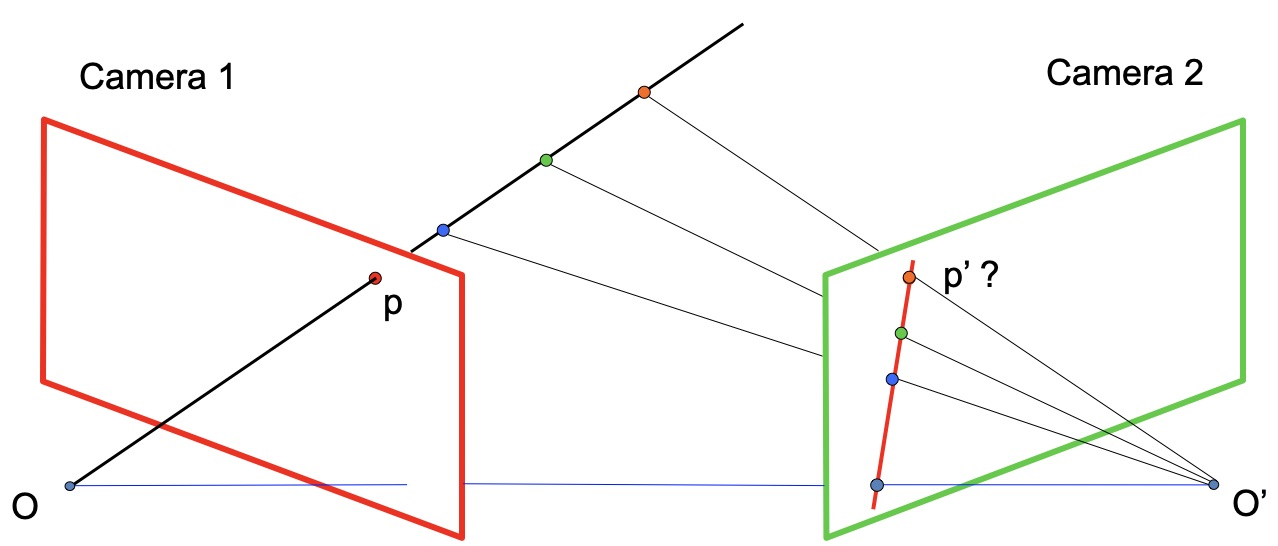
\includegraphics[width=0.8\linewidth]{figures/stereo/epipolar.jpg}
}
\caption{Epipolar lines}
\label{fig:epipolar}
\end{figure}

Knowing where to look for the match for a given feature point in another image can greatly reduce the computational complexity and increase the reliability of the task.  Figure~\ref{fig:epipolar} shows the geometry of the matching task.  A given feature at location p in camera 1 can occur anywhere in depth along the line connecting O (the optical center of camera 1) and the location of the feature point in the virtual sensor point, p.  When each possible 3d point is viewed from camera 2, those points will appear on the sensor plane of the camera where the line connecting them from each possible 3d position to the optical center of camera 2, O', intersects the virtual sensor plane of camera 2.  All points from the line Op to the point O' form a plane.  Except for degenerate configurations, the intersection of that plane with the sensor plane of camera 2 will form a line, which is called an epipolar line.  To find the stereo match for the point p, we only need to look along the  epipolar line in the image formed by camera 2.





\section{Imaging Geometry}
The example of Fig.~\ref{fig:stereo} is a special case, parallel, identical cameras, of the general stereo problem.  To infer depth from a more general pair of stereo images, we need to know the relationship between the positions of points in the world and where they appear in the images from each camera.  Determining those relationships, which involves both measuring properties of the cameras and also their positions and orientations, is called {\em camera calibration}.
Often the image pairs are pre-distorted to ensure that horizontal disparity 
corresponds to object depth, a step known as {\em rectification}.
To perform the calculations needed for camera calibration it is convenient to use a set of coordinates known as homogeneous coordinates.

\subsection{Homogenous Coordinates}
The perspective projection equations, relating camera pixel position of the image of a point to the point's world 3-d position, involve division by the point's Z location, as in Eq.~(\ref{eq:perspectiveProj}).  This division complicates algebraic relations.  Projective geometry and homogeneous coordinates are tools that simplify those algebraic relations, and thus simplify the camera calibration calculations.

Conventional Cartesian coordinate descriptions of a point in 2-d, such as $(x,y)$, or 3d, such as $(x,y,z)$, we will refer to as heterogenous coordinates.  We denote their corresponding homogeneous coordinate representations by square bracketed vectors and are:
\begin{equation}
    (x,y) \rightarrow 
    \left [
    \begin{array}{c}
    x \\
    y \\
    1
    \end{array}
    \right ]
    \label{eq:2dhomo}
\end{equation}
and
\begin{equation}
    (x,y,z) \rightarrow 
    \left [
    \begin{array}{c}
    x \\
    y \\
    z \\
    1
    \end{array}
    \right ]
    \label{eq:3dhomo}
\end{equation}
The transformation rule from heterogeneous to homogeneous coordinates is simply to add an additional coordinate, 1, to the heterogenous coordinates, with the additional rule that all scalings of a homogenous coordinate vector are equivalent.  To go from homogeneous coordinates back to the heterogenous representation of the point, we divide all the entries of the homogenous coordinate vector by it's last dimension.  For example, to represent a 2-d point, we have (transforming from heterogenous to homogeneous coordinates):
\begin{equation}
    (x,y) \rightarrow 
        \left [
    \begin{array}{c}
    x \\
    y \\
    1
    \end{array}
    \right ]
    =
        \left [
    \begin{array}{c}
    a x \\
    a y \\
    a
    \end{array}
    \right ]
\end{equation}
for any non-zero scalar, a.
We also have (transforming from homogenous to heterogeneous coordinates):
\begin{equation}
        \left [
    \begin{array}{c}
    x \\
    y \\
    w
    \end{array}
    \right ]
    \rightarrow 
     \left ( \frac{x}{w}, \frac{y}{w} \right )
\end{equation}


We'll explore these for 2d geometry first, then see how they can represent 3d perspective projection easily.



\subsection{2D Transformations}
\label{sect:2dtransforms}
Common transformations we'll want to represent include:  translation, rotation, scaling, and shearing.
\subsubsection{Translation}
Consider a translation by a 2d vector, $(t_x, t_y)$. We'll denote the coordinates after the transformation with a prime. In heterogenous coordinates, we have
\begin{equation}
        \left (
    \begin{array}{c}
    x' \\
    y' 
    \end{array}
    \right )
    =
            \left (
    \begin{array}{c}
    x \\
    y 
    \end{array}
    \right )
    +
            \left (
    \begin{array}{c}
    t_x \\
    t_y 
    \end{array}
    \right )
\end{equation}
We can write this translation in homogeneous coordinates by
\begin{equation}
            \left (
    \begin{array}{c}
    x' \\
    y' \\
    1
    \end{array}
    \right )
    =
            \left (
    \begin{array}{ccc}
    1 & 0 & t_x \\
    0 & 1 & t_y \\
    0 & 0 & 1
    \end{array}
    \right )
            \left (
    \begin{array}{c}
    x \\
    y \\
    1
    \end{array}
    \right )
\end{equation}
Writing the equation above in terms of vector points $\mathbf{p}$, we have
\begin{equation}
    \mathbf{p}' = T \mathbf{p},
\end{equation}
with the homogenous matrix, $\mathbf{T}$, defined as
\begin{equation}
    \mathbf{T} =             \left (
    \begin{array}{ccc}
    1 & 0 & t_x \\
    0 & 1 & t_y \\
    0 & 0 & 1
    \end{array}
    \right )
\end{equation}
For calculations in homogeneous coordinates, both matrices and vectors are only defined up to an arbitrary multiplicative scaling factor.

To cascade two translation operations $\mathbf{t}$ and  $\mathbf{s} $, in heterogeneous coordinates, we have
\begin{equation}
     \mathbf{p}' = \mathbf{p} + \mathbf{t}  + \mathbf{s}    
\end{equation}

In homogeneous coordinates, we cascade the corresponding translation matrices:
\begin{equation}
     \mathbf{p}' = S T \mathbf{p},
\end{equation}
where the homogenous translation matrix, $\mathbf{S}$, corresponding to the offset $\mathbf{s}$, is:
\begin{equation}
    \mathbf{S} =             \left (
    \begin{array}{ccc}
    1 & 0 & s_x \\
    0 & 1 & s_y \\
    0 & 0 & 1
    \end{array}
    \right )
\end{equation}


\subsubsection{Rotation}
For a rotation by an angle $\theta$, we simply have the matrix
\begin{equation}
    \mathbf{R} =             \left (
    \begin{array}{ccc}
    \cos(\theta) & \sin(\theta) & 0 \\
    -\sin(\theta) & \cos(\theta & 0 \\
    0 & 0 & 1
    \end{array}
    \right )
\end{equation}


\subsubsection{Scaling}
Scaling the x-axis by $s_x$ and the y-axis by $s_y$ yields the transformation matrix,
\begin{equation}
    \mathbf{S} =             \left (
    \begin{array}{ccc}
    s_x & 0 & 0 \\
    0 & s_y & 0 \\
    0 & 0 & 1
    \end{array}
    \right )
\end{equation}

\subsubsection{Shearing}
Shearing involves scale factors in the off-diagonal matrix locations, as shown in the matrix, $\mathbf{Q}$:
\begin{equation}
    \mathbf{Q} =             \left (
    \begin{array}{ccc}
    1 & q_x & 0 \\
    q_y & 1 & 0 \\
    0 & 0 & 1
    \end{array}
    \right )
\end{equation}


\subsection{Camera Projections}
To write points in 3-d space in homogeneous coordinates, we add a 4th coordinate to the three of Euclidean space, with the same scaling rules applying as for the case of 2-d homogeneous coordinates.
Using homogeneous coordinates, camera projections can be written in a simple form as a matrix multiplication.  Consider a coordinate system with the origin fixed at the center of projection of the camera and the 3d point, in homogeneous coordinates:
\begin{equation}
        \mathbf{P} = 
            \left [
    \begin{array}{c}
    x \\
    y \\
        z \\
    1
    \end{array}
    \right ]
\end{equation}
We can verify that the matrix, $\mathbf{V}$, shown below, multiplied by the vector describing the 3d point, $\mathbf{p}$, above, returns the position of its perspective projection, Eq.~(\ref{eq:perspctiveProj}):
\begin{eqnarray}
        \mathbf{V} \mathbf{p} & = &
         \left [
    \begin{array}{cccc}
    1 & 0 & 0 & 0 \\
    0 & 1 & 0 & 0 \\
    0 & 0 & \frac{1}{f} & 0
    \end{array}
    \right ]
            \left [
    \begin{array}{c}
    X \\
    Y \\
        Z \\
    1
    \end{array}
    \right ] \\
    & = & 
     \left [
    \begin{array}{c}
    X \\
    Y \\
        \frac{Z}{f}
    \end{array}
    \right ]
\end{eqnarray}
Transforming the product vector from homogeneous coordinates to heterogeneous coordinates yields
\begin{equation}
         \left [
    \begin{array}{c}
    X \\
    Y \\
        \frac{Z}{f}
    \end{array}
    \right ]
    \rightarrow
             \left (
    \begin{array}{c}
    \frac{f X}{Z} \\
    \frac{f Y}{Z}
    \end{array}
    \right ),
\end{equation}
showing that the matrix $\mathbf{V}$, when multiplied by the homogeneous coordinates of a 3d point, renders the homogeneous coordinates of the perspective projection of that 3d point.

Because homogeneous coordinates, and therefore also the transformation matrices, are only defined up to an arbitrary uniform scale factor, the perspective projection transformation matrix is sometimes equivalently written as,
\begin{equation}
    \mathbf{V} =             \left [
    \begin{array}{cccc}
    f & 0 & 0 & 0 \\
    0 & f & 0 & 0 \\
    0 & 0 & 1 & 0
    \end{array}
    \right ]
    \label{eq:homogPerspective}
\end{equation}


The projection matrix for an orthographic projection, Eq.~(\ref{eq:orthographicProj}), $\mathbf{W}$, is
\begin{equation}
\mathbf{W} =         \left [
    \begin{array}{cccc}
    1 & 0 & 0 & 0 \\
    0 & 1 & 0 & 0 \\
    0 & 0 & 0 & 1
    \end{array}
    \right ],
\end{equation}
as can be verified by multiplying by a 3d point in homogeneous coordinates.


\section{Camera Parameters}
A camera is said to be {\em calibrated} if we know how to convert from 3d world coordinates to pixel coordinates within the camera. That conversion involves two types of parameters:  (1) parameters that depend on where the camera is physically located in the world, and (2) parameters that are a function of the camera itself.  These two types of parameters are called extrinsic and intrinsic parameters, respectively.


\subsection{Camera Extrinsic Parameters}
First, we need to translate, and then to rotate the camera so that points in the world, $\mathbf{p}_W$, are written in terms of a coordinate system with its origin at the camera center, and rotated to align with the camera.  To do so, we first translate the coordinate system by $-\mathbf{T}$ using the homogeneous matrix, $\mathbf{M}_1$, where $\mathbf{T}$ is the position of the camera in world coordinates:
\begin{equation}
\mathbf{M}_1 =         \left [
    \begin{array}{cccc}
    1 & 0 & 0 & -T_X \\
    0 & 1 & 0 & -T_Y \\
    0 & 0 & 1 & -T_Z \\
    0 & 0 & 0 & 1
    \end{array}
    \right ]
\end{equation}
Then, we use the 3x3 matrix, $\mathbf{R}$, to rotate the camera so that the camera's coordinates are parallel to those of the world:
\begin{equation}
\mathbf{M}_2 =         \left [
    \begin{array}{cccc}
    R_1 & R_2 & R_3  & 0 \\
    R_4 & R_5 & R_6 & 0 \\
    R_7 & R_8 & R_9 & 0 \\
    0 & 0 & 0 & 1
    \end{array}
    \right ]
    \label{eq:homographyRotation}
\end{equation}
We have
\begin{equation}
\mathbf{p}_C = \mathbf{M}_2 \mathbf{M}_1 \mathbf{p}_W
\label{eq:extrinsic}
\end{equation}
where $\mathbf{p}_W$ and $\mathbf{p}_C$ are the coordinates of the same point, written in world and camera  coordinates, respectively.


\subsection{Camera Intrinsic Parameters}
Now we need to account for the perspective projection of the point, $\mathbf{p}_C$, described in camera coordinates, to pixel coordinates in the sensor plane of the camera.  The units of the position in pixel space may be different than those of the world coordinates, introducing a scaling of the focal length, f, in Eq.~(\ref{eq:homogPerspective}) to another value, call it a:
\begin{equation}
    \mathbf{M}_3 =             \left [
    \begin{array}{cccc}
    a & 0 & 0 & 0 \\
    0 & a & 0 & 0 \\
    0 & 0 & 1 & 0
    \end{array}
    \right ]
    \label{eq:intrinsic}
\end{equation}

The concatenation of the extrinsic and intrinsic transformation matrices  yields the desired transformation matrix which will convert world coordinates to rendered pixel coordinates:
\begin{equation}
        \left [
    \begin{array}{c}
    x \\
    y \\
    w
    \end{array}
    \right ] 
=
\mathbf{M}_3 \mathbf{M}_2 \mathbf{M}_1 
        \left [
    \begin{array}{c}
    X \\
    Y \\
    Z \\
    1
    \end{array}
    \right ] 
    \label{eq:combined}
\end{equation}
Converting back to heterogeneous from homogeneous coordinates, the pixel indices of a point $(X, Y, Z)$ in the world will be $(\frac{x}{w}, \frac{y}{w})$.

Writing this out, we have, for the case of simplified camera intrinsic parameters (square pixels), but general extrinsic parameters, the expression to transform from 3d position to the measured sensor position of that 3d point:
\begin{equation}
        \left [
    \begin{array}{c}
    x \\
    y \\
    w
    \end{array}
    \right ] 
=
 \left [
    \begin{array}{cccc}
    a & 0 & 0 & 0 \\
    0 & a & 0 & 0 \\
    0 & 0 & 1 & 0
    \end{array}
    \right ]
     \left [
    \begin{array}{cccc}
    R_1 & R_2 & R_3  & 0 \\
    R_4 & R_5 & R_6 & 0 \\
    R_7 & R_8 & R_9 & 0 \\
    0 & 0 & 0 & 1
    \end{array}
    \right ]
     \left [
    \begin{array}{cccc}
    1 & 0 & 0 & -T_X \\
    0 & 1 & 0 & -T_Y \\
    0 & 0 & 1 & -T_Z \\
    0 & 0 & 0 & 1
    \end{array}
    \right ]
        \left [
    \begin{array}{c}
    X \\
    Y \\
    Z \\
    1
    \end{array}
    \right ] 
    \label{eq:combinedexpanded}
\end{equation}
The right-most matrix multiplications reflect the camera's extrinsic parameters, and the left-most matrix reflects the intrinsic parameters and the perspective projection.  Note that column of zeros in the left-most matrix means that, without loss of generality, Eq.~(\ref{eq:combinedexpanded}) can be written in slightly simpler form as:
\begin{equation}
        \left [
    \begin{array}{c}
    x \\
    y \\
    w
    \end{array}
    \right ] 
=
 \left [
    \begin{array}{ccc}
    a & 0 & 0  \\
    0 & a & 0  \\
    0 & 0 & 1 
    \end{array}
    \right ]
     \left [
    \begin{array}{cccc}
    R_1 & R_2 & R_3  & 0 \\
    R_4 & R_5 & R_6 & 0 \\
    R_7 & R_8 & R_9 & 0
    \end{array}
    \right ]
     \left [
    \begin{array}{cccc}
    1 & 0 & 0 & -T_X \\
    0 & 1 & 0 & -T_Y \\
    0 & 0 & 1 & -T_Z
    \end{array}
    \right ]
        \left [
    \begin{array}{c}
    X \\
    Y \\
    Z \\
    1
    \end{array}
    \right ] 
    \label{eq:combinedexpandedsmaller}
\end{equation}

\section{Homography}

We can use the tools of homogeneous coordinates and camera calibration described above to address image stitching and for image rectification to simplify stereo calculations. We describe each in turn.

\subsection{Image Stitching}
A far-away scene may not fit into the field of view of a camera, and photographers often choose to take multiple photos of the scene, allowing the camera or special software to warp and stitch together each photograph into a large panorama.  How should we warp the images to let them fit together as seamlessly as possible?

For the case of multiple photographs from a hand-held camera, in general, there will be both translation and rotation between the photographs.  However, if the scene is sufficiently far away, the effect on the image of the spatial translation of the camera will be negligible, and we can consider the multiple images to be stitched together as sharing the same optical center, and differing only in the camera's orientation.

Here, we show that the mapping between feature point locations in two cameras differing only in their 3d orientation is 3x3 matrix transformation of their 2-d positions written in homogeneous coordinates, called a homography. Setting the translation vector to be zero in Eq.~\ref{eq:combinedexpandedsmaller}, and writing the $3\times3$ rotation matrices for camera 1 as $\mathbf{R_1}$ and $\mathbf{R_2}$, respectively, we have for the observed position of a common 3d point observed from camera 1:
\begin{equation}
        \left [
    \begin{array}{c}
    x_1 \\
    y_1 \\
    w_1
    \end{array}
    \right ] 
=
 \left [
    \begin{array}{ccc}
    a & 0 & 0  \\
    0 & a & 0  \\
    0 & 0 & 1 
    \end{array}
    \right ]
     \left [
    \begin{array}{cccc}
     &  &   & 0 \\
     & \mathbf{R_1} &  & 0 \\
     &  &  & 0
    \end{array}
    \right ]
        \left [
    \begin{array}{c}
    X \\
    Y \\
    Z \\
    1
    \end{array}
    \right ] 
    \label{eq:camera1}
\end{equation}
Left-multiplying Eq.~(\ref{eq:camera1}) by 
$\mathbf{R_1}^{-1} 
\left [
    \begin{array}{ccc}
    a^{-1} & 0 & 0  \\
    0 & a^{-1} & 0  \\
    0 & 0 & 1 
    \end{array}
    \right ] $,
    and doing the same for the analogous equations for camera 2, yields:
 \begin{equation}
 \mathbf{R_1}^{-1}
 \left [
    \begin{array}{ccc}
    a^{-1} & 0 & 0  \\
    0 & a^{-1} & 0  \\
    0 & 0 & 1 
    \end{array}
    \right ]
        \left [
    \begin{array}{c}
    x_1 \\
    y_1 \\
    w_1
    \end{array}
    \right ] 
=
 \mathbf{R_2}^{-1}
 \left [
    \begin{array}{ccc}
    a^{-1} & 0 & 0  \\
    0 & a^{-1} & 0  \\
    0 & 0 & 1 
    \end{array}
    \right ]
        \left [
    \begin{array}{c}
    x_2 \\
    y_2 \\
    w_2
    \end{array}
    \right ] 
    \label{eq:homo1}
\end{equation}   
This leads to:
 \begin{eqnarray}
        \left [
    \begin{array}{c}
    x_1 \\
    y_1 \\
    w_1
    \end{array}
    \right ] 
    & =  &
 \left [
    \begin{array}{ccc}
    a & 0 & 0  \\
    0 & a & 0  \\
    0 & 0 & 1 
    \end{array}
    \right ]
 \mathbf{R_1}
 \mathbf{R_2}^{-1}
 \left [
    \begin{array}{ccc}
    a^{-1} & 0 & 0  \\
    0 & a^{-1} & 0  \\
    0 & 0 & 1 
    \end{array}
    \right ]
        \left [
    \begin{array}{c}
    x_2 \\
    y_2 \\
    w_2
    \end{array}
    \right ] 
    \label{eq:homo2} \\
       & =  &
\mathbf{H}
        \left [
    \begin{array}{c}
    x_2 \\
    y_2 \\
    w_2
    \end{array}
    \right ] 
    \label{eq:homo3} 
\end{eqnarray}   
where $\mathbf{H}$ is a $3\times3$  matrix.  Thus, camera rotation modifies the locations of the image points by a homography. To stitch together images, one typically estimates the homography through solving Eq.~(\ref{eq:homogeneous}), rather than through estimating the rotation and intrinsic camera matrices within Eq.~(\ref{eq:homo3}).


Thus, an additional transformation to add to the 2-d transformations of Section~\ref{sect:2dtransforms} is a homography, given by a general 3x3 matrix transformation of homographic coordinates:
\begin{equation}
    \mathbf{H} =             
    \left (
    \begin{array}{ccc}
    a & b & c \\
    d & e & f \\
    g & h & i
    \end{array}
    \right )
\end{equation}


Under certain conditions, a homography predicts the position of points when viewed with another camera from another position. We just discussed one condition, when the two cameras have the same focal length and just differ in their position and orientation by a rotation about the center of projection.  A second case, it can be shown \cite{Hartley2004}, is when the 3d shape of the observed image is a plane.  For either condition, we may want to compute the homography transformation from the two images.  

Given a set of feature point locations, and their correspondences across the two cameras, we can compute the homography relating the locations of imaged points within the two cameras.  Consider the $i$th pair of feature point locations, rendered at position (x,y,w) in homogeneous coordinates in the first camera and at position (x',y',w') in the second.  Because the two homogeneous coordinate vectors, and the homography relating them, are all defined only to within a multiplicative constant, without loss of generality, we can set w=1.  Then we have, for the $i$th matching feature points,
\begin{equation}
              \left [
    \begin{array}{c}
    x_i' \\
    y_i' \\
    w_i' 
    \end{array}
    \right ]           
    \left [
    \begin{array}{ccc}
    a & b & c \\
    d & e & f \\
    g & h & i
    \end{array}
    \right ]
    \left [
    \begin{array}{c}
    x_i \\
    y_i \\
    1 
    \end{array}
        \right ] 
        \label{eq:homo1}
\end{equation}

Converting Eq.~(\ref{eq:homo1}) to heterogeneous coordinates yields the constraint,
\begin{eqnarray}
        x_i' & = & \frac{a x_i + b y_i + c}{g x_i h y_i + i} \\
        y_i' & = & \frac{d x_i + e y_i + f}{g x_i h y_i + i} 
\end{eqnarray}
Rearranging terms, we have these two constraints from the $i$ feature point pair:
\begin{eqnarray}
        g x_i x_i' +  h y_i x_i' + i x_i' -a x_i - b y_i - c  = 0 \\
           \label{eq:constraints1}
        g x_i y_i' +  h y_i y_i' + i x_i' -d x_i - e y_i - f = 0
        \label{eq:constraints2}
\end{eqnarray}
The equations Eq.~(\ref{eq:constraints1}) and Eq.~(\ref{eq:constraints2}) above, for all $i = 1 \ldots N$, where $N$ is the number of feature point pairs can be written compactly in matrix form,
\begin{equation}
    \mathbf{A} \mathbf{h} = 0
    \label{eq:homogeneous}
\end{equation}
where $\mathbf{h}$ contains the terms $a \ldots i$ stacked into a vector.  This homogeneous least squares problem can be solved for the unit norm values of the best-fitting homography matrix parameters (stacked into the vector elements of $\mathbf{h}$) by finding the right singular vector corresponding to the smallest singular value of the matrix, $\mathbf{A}$ \cite{Forsyth2012}.

\subsubsection{Robust model fitting--RANSAC}
To perform the image stitching in the section above, we had to find the homography parameters that best described the transformation from one image to another. Because the detection of the feature points can be noisy, the homography fitting needs to be robust against feature mis-matches between images.  A good algorithm to fit models to data robustly is  RANSAC \cite{Fischler1981}, which stands for RANdom SAmpling with Concensus.  Introduced in 1981, it has been a workhorse in computer vision over the years since \cite{Zisserman2006}.

The procedure for RANSAC is simple, and the name contains most of the steps of the algorithm.  First, RANdomly select a sufficient set of datapoints to fit the parameters of some model.  The could be the parameters that define a line, some other structure, or a homography.  Then, compute the model parameters from the randomly SAMpled set of points. Compute the inliers in the dataset--the datapoints that fit the model (or achieve Consensus) to within some tolerance.  Repeat that procedure some number of times, $N$.    Compute a final model from the set of inlier points corresponding to the largest number of inlier datapoints.

Figure~\ref{fig:ransac} shows a simple instantiation of this algorithm for the case of robustly fitting a straightline model to a collection of datapoints, Fig.~\ref{fig:ransac}~(a).  First, a number of datapoints, sufficient to uniquely specify the model parameters, are drawn from the dataset.  For this problem, that is two points.  Two randomly selected points are marked in green in Fig.~\ref{fig:ransac}~(b).  After finding the line that passes through those two points, the number of "inliers"--datapoints within $\epsilon$ of the model--is determined.  For the line of (b), the number of inliers is three. This process is repeated

The authors derive a heuristic for the number of samples, S, required to be assured a good model fit.  Let n be the number of datapoints required to specify the model, and let w be (an estimate of) the probability that any selected datapoint is within the error tolerance of the model.   For the example of Fig.~\ref{fig:ransac}, as seen in (f), there are n=2 outliers out of 11 points, so w = 0.18 (in general, this value needs to be estimated).  $w^n$ is the probability that all the selected points are inliers, and $1 -  w^n$ is the probability that at least one selected point is an outlier.  The probability that in k trials only bad models are selected is then $(1 -  w^n)^k$.  I $p$ is the probability of selecting the correct model, we have (see also \cite{wikiRANSAC}
\begin{equation}
    1-p = (1 -  w^n)^k
\end{equation}
Taking the logarithm of both sides lets us solve for k, the number of RANSAC iterations required to find a good fit, with probability $p$:
\begin{equation}
        k = \frac{\log(1-p)}{\log(1-w^n)}
        \label{eq:k}
\end{equation}
For the example of Fig.~\ref{fig:ransac}, for 95\% accuracy, $k = \frac{\log(-05)}{\log(1-0.18^2)} = \frac{-1.3}{-0.0143} = 91$
So with 91 trials, we would have 95\% confidence of finding the correct model through RANSAC. 


\begin{figure}
\centerline{
\sublabel{a}{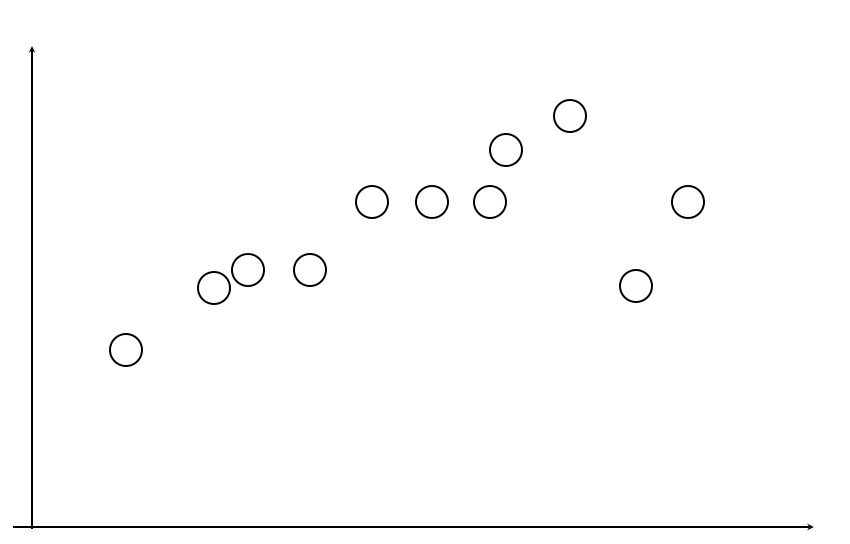
\includegraphics[width=0.4\linewidth]{figures/stereo/ransac1.jpg}}
\sublabel{b}{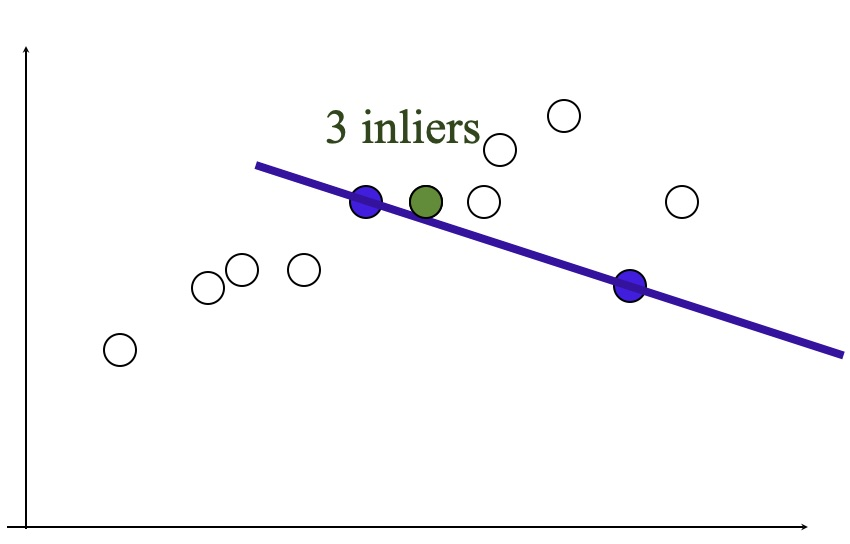
\includegraphics[width=0.4\linewidth]{figures/stereo/ransac2.jpg}}}
\centerline{
\sublabel{c}{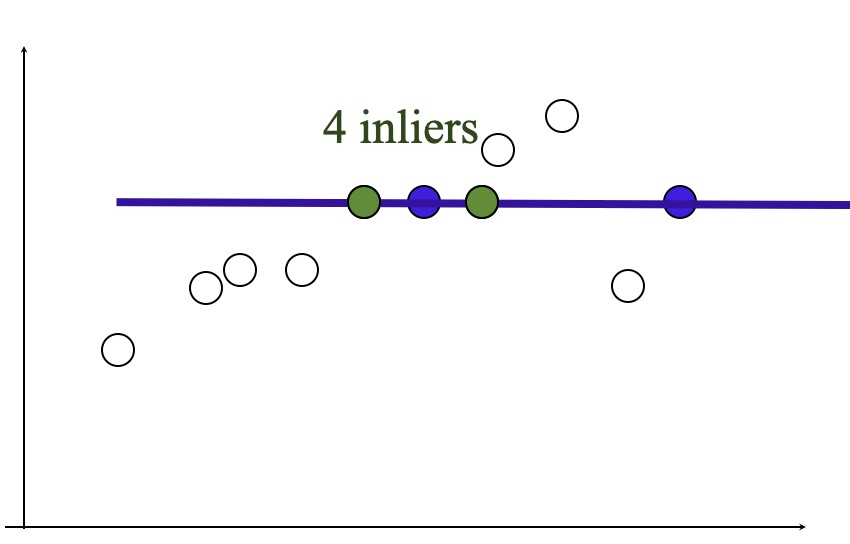
\includegraphics[width=0.4\linewidth]{figures/stereo/ransac3.jpg}}
\sublabel{d}{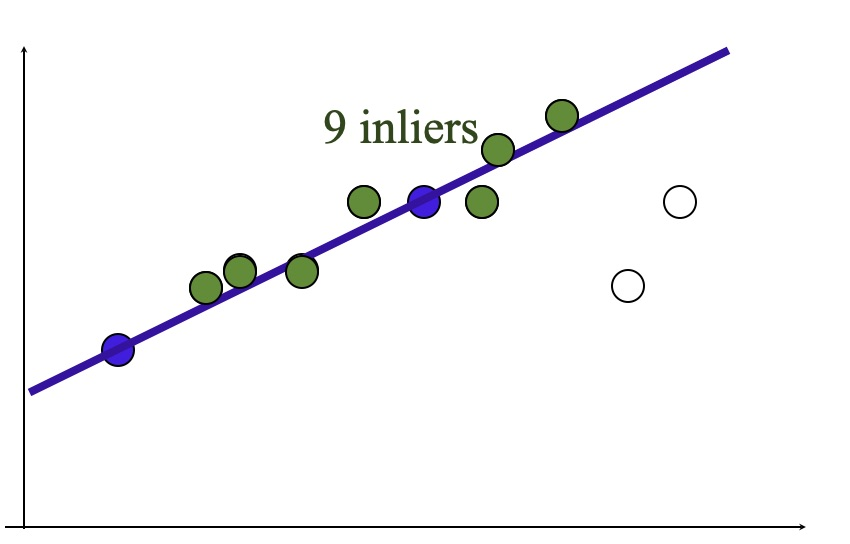
\includegraphics[width=0.4\linewidth]{figures/stereo/ransac4.jpg}}}
\centerline{
\sublabel{e}{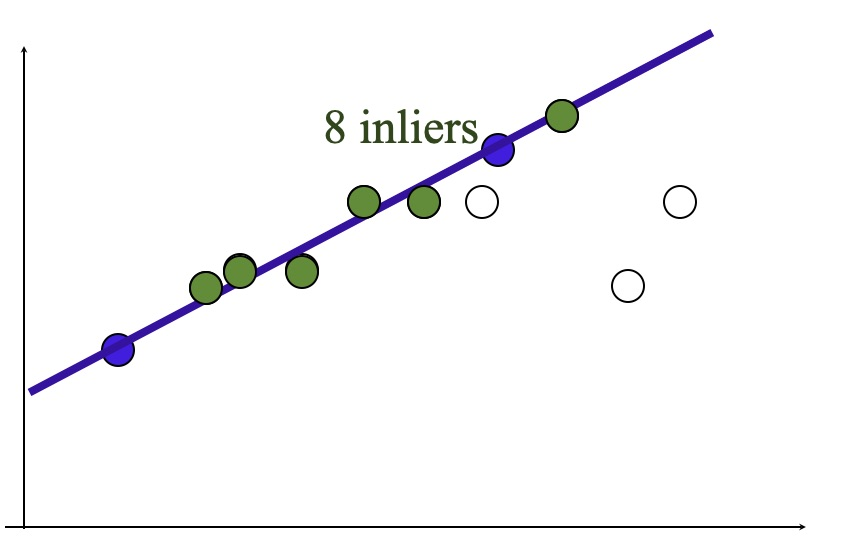
\includegraphics[width=0.4\linewidth]{figures/stereo/ransac5.jpg}}
\sublabel{f}{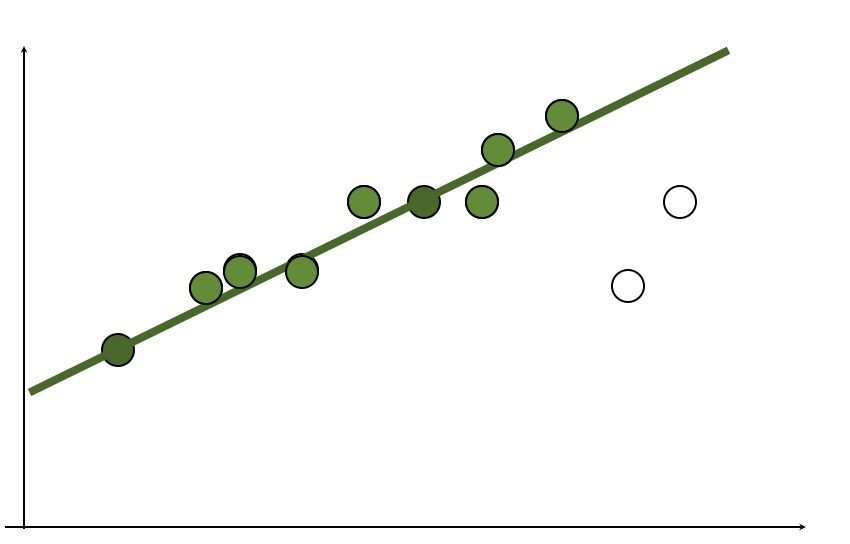
\includegraphics[width=0.4\linewidth]{figures/stereo/ransac6.jpg}}}
\caption{RANSAC applied to robust estimation of line parameters. (a) datapoints for which robust line estimation is sought. (b) two points (in blue) are selected at random, sufficient to estimate line model parameters. The number of inliers is computed for this model. (c) - (e) repeat k times. (f) select the model with the maximum number of inliers.}
\label{fig:ransac}
\end{figure}



The RANSAC loop applied to fitting a homography, to within probability $p$, is:
\begin{enumerate}
\item Repeat k times (Eq.~(\ref{eq:k})):
\begin{enumerate}
\item Select four (n = 4) feature pairs (at random).
\item Compute homography H (exact).
\item Compute inliers where $||pi’, H pi|| < ε $ .
\end{enumerate}
\item Keep largest set of inliers.
\item Re-compute least-squares H estimate using all of the inliers.
\end{enumerate}




\subsection{Image rectification}
Another application of homography transformations is the stereo pre-processing step called {\em image rectification}.  As described above, one only needs to search along epipolar lines to find matching points in the second image.  If the sensor planes of each camera are co-planar, and if the pixel rows are co-linear across the two cameras, then the epipolar lines will be along image scanlines, simplifying the stereo search.  Using the homography transformations, we can warp the stereo camera images to synthesize the images that would be recorded from cameras aligned in that way.

Many configurations of the two cameras satisfy the two image rectification constraints \cite{Zhang2003}, that epipolar lines are along image scanlines, and matching points are within the same rows in each camera image.  One algorithm that will satisfy those constraints is as follows \cite{wikiRectification}:  


First, use Eq.~(\ref{eq:homographyRotation}) to rotate each camera to be parallel with each other and pointing away from the line joining the two camera centers.  Second, rotate each of the cameras about its optical axis to align the rows of each camera with those of the other.  Third, uniformly scale one camera's image to be the same size as to the other, if necessary.  The resulting image pair will satisfy the requirements for image rectification.

Others algorithms are optimized to minimize image distortions \cite{Zhang2003} and may give better performance for stereo algorithms.  We assume camera calibrations are known, but other rectification algorithm can require only weaker conditions, such as knowing the fundamental matrix \cite{Hartley2004}. Many software packages provide image rectification code.

\section{Comparing the performance of stereo algorithms}
The "Middlebury Stereo web page" \cite{Scharstein2002} provides a comprehensive comparison of many stereo algorithms, compared on a common dataset, with pointers to algorithm descriptions and code.  One can use the web page to evaluate the improvement of stereo reconstruction algorithms over time.  The advancement of the field over time is very impressive.


